\begin{quote}
    \textit{``Not only are we going to make our cow spherical, we're going to shoot it down so it doesn't move.'' --Jorge Santos}
\end{quote}

So far, we discussed two key concepts. We discussed the condition of a spacetime being static, i.e. stationary and enjoying invariance under $t\leftrightarrow -t$, which forced the line element to take the form
\begin{equation}
    ds^2 = g_{tt}(x^k)dt^2 + g_{ij}(x^k)dx^i dx^j.
\end{equation}
%not only are we going to make our cow spherical, we're going to shoot it down so it doesn't move.
We also required spherical symmetry, i.e. the $SO(3)$ orbits of points $p$ in the manifold are $S^2$s.

Let us see what we get when we combine static and spherically symmetric solutions. We know from staticity that there is a timelike Killing vector $K=\left(\P{}{t}\right)^a$. Suppose we take a hypersurface $\Sigma_t$ which is normal to our timelike Killing vector $K$. Then take any point $p\in \Sigma_t$. By spherical symmetry, its $SO(3)$ orbit is a sphere $S^2$. Assign angular coordinates $\theta,\phi$ on the $S^2$ orbit. Using spacelike geodesics normal to the sphere $S^2$, we can then extend $\theta,\phi$ to the entire hypersurface, a process which is shown in Fig. \ref{fig:sphericalcoords}.

\begin{figure}
    \centering
    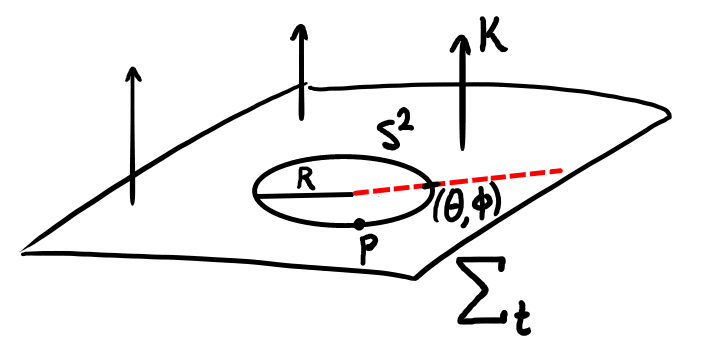
\includegraphics[width=0.75\textwidth]{2019/01/20190121_sphericalcoords.png}
    \caption{An illustration of our coordinates for static, spherically symmetric solutions. We can always choose a hypersurface $\Sigma_t$ which is orthogonal to the timelike Killing vector $K$. On $\Sigma_t$, choose a point $p$ and trace out its $S^2$ orbit (drawn here as a circle, $S^1$) under the action of the $SO(3)$ symmetry. On the $S^2$ orbit, we can define angular coordinates $(\theta,\phi)$, and we can then extend these to the rest of $\Sigma_t$ by defining $\theta,\phi$ to be constant on spacelike geodesics normal to the $S^2$ orbit (red dashed line). The radial coordinate $r$ is given by the area formula $r=\sqrt{A(p)/4\pi}.$ This defines coordinates on $\Sigma_t$, which we can extend to the entire manifold by following the integral curves of $K$.}
    \label{fig:sphericalcoords}
\end{figure}

Thus our metric on $\Sigma_t$ takes the form
\begin{equation}
    ds^2_{\Sigma_t}=e^{2\psi(r)}dr^2 +r^2 d\Omega^2_2,
\end{equation}
where the coefficient of $dr^2$ must only depend on $r$ by spherical symmetry, and $r$ is given by our old area relation, $r:\cM\to \RR^+$ with $r(p)=\sqrt{\frac{A(p)}{4\pi}}$. Now using the property our spacetime is static, we can write down the full spacetime metric,
\begin{equation}
    ds^2= -e^{2\Phi(r)}dt^2 +ds^2_{\Sigma_t}.
\end{equation}
So far we have two degrees of freedom, $(\psi(r),\Phi(r)).$ Let's now put some physics in and consider a fluid in our spherically symmetric spacetime. For fluids, recall that the stress-energy tensor takes the form
\begin{equation}
    T_{ab}=(\rho+p)U_a U_b + pg_{ab}
\end{equation}
where $U_a$ is a four-velocity, $\rho$ is an energy density and $p$ is a pressure. By spherical symmetry, $\rho$ and $p$ can only be functions of the radial coordinate $r$, so $\rho=\rho(r)$ and $p=p(r)$. The four-velocity is always timelike, so
\begin{equation}
    U^a U_a = U^a U^b g_{ab}=-1 %\implies U_t^2 g^{tt} = -1 
        \implies U^a = e^{-\Phi}\paren{\P{}{t}}^a
\end{equation}
so that $p,\rho >0$. This is an energy condition.
%Completely vacuous statement so far. Literally! Since it is in vacuum.

We want to describe spherical stars (with finite spatial extent), so outside the star both the pressure and energy density must vanish,
\begin{equation}
    p=\rho = 0\text{ for }r > R
\end{equation}
with $R$ the radius of the star. Now, we know that the defining property of stress-energy is that it is conserved-- $\nabla^a T_{ab}=0$. But the Einstein equation says that
\begin{equation}
    R_{ab}-\frac{R}{2}g_{ab}=T_{ab},
\end{equation}
and by the contracted Bianchi identity we know that the divergence of the LHS always vanishes, so it suffices to look at the Einstein equation since it automatically implies the conservation equation for fluids. This is not generally true for other energy content since there may be other equations of motion that apply.

Let's look at a specific example, the $tt$ component of the Einstein equations.
\begin{equation}
    G_{tt}=\frac{e^{2(\Phi-\psi)}}{r^2}\bkt*{e^{2\psi}+2r \psi' -1},
\end{equation}
where the prime indicates a $\P{}{R}$.

Let us also define a function $m(r)$, given by
\begin{equation}
    e^{2\psi}\equiv \bkt{1-\frac{2m(r))}{r}}^{-1}.
\end{equation}
From the various components we learn that
\begin{align}
    tt: m' &= 4\pi r^2 \rho(r)\\
    nn: \Phi' &= \frac{m+4\pi r^3 p}{r(r-2m)}\\
    \theta\theta : p' &= -(p+\rho)\frac{m + 4\pi n^3 p}{r[r-2m(r)]}.
\end{align}
We call these the Tollman-Oppenheimer-Volkoff equations (TOV for short).
We have three equations but four unknowns: $m, \Phi, p$ and $\rho$. We need one more bit of information-- namely, an equation of state relating the pressure and energy density. Normally, $p$ depends on $\rho$ and also $T$ the temperature. But for our purposes, we will assume cold stars so that $p$ is only a function of the energy density $\rho$.

What can we figure out before imposing any sort of conditions on $p(\rho)$? Well, outside the star, $r>R,$ we have $p=\rho=0.$ But we see immediately that in the region $\rho=0$, the $tt$ equation tells us that $m'=0\implies m=M$ for some constant $M$. This in turn implies that
\begin{equation}
    \psi(r)=-\frac{1}{2}\log\paren{1-\frac{2M}{r}} = -\Phi(r).
\end{equation}
We can now write down the line element in the exterior region,
\begin{equation}
    ds^2=-\paren{1-\frac{2M}{r}}dt^2 +\frac{dr^2}{1-\frac{2M}{r}} + r^2 d\Omega_2^2.
\end{equation}
This is the \term{Schwarzschild line element.} We identify the parameter $M$ with the mass of the system.

There's a bit of physics to extract from this-- for \emph{stars}, we need $R>2M$ to keep the signs correct in the metric. For the sun, we have $2M_\odot = \SI{3}{\kilo\meter}$ and $R\simeq \SI{7e5}{\kilo\meter},$ so this is a (very loose) bound which is easily satisfied.

Inside the star, life is not so easy. The mass now depends on the radius, and it has a solution
\begin{equation}
    m(r)=4\pi \int_0^r \rho(\tilde r) \tilde r^2 d\tilde r + m_*,
\end{equation}
with $m_*$ some integration constant. Fortunately, we note that by physical concerns, $m(r)\to 0$ as $r\to 0$ in order to preserve regularity (the metric should look flat), which tells us that this integration constant is zero, $m_*=0$.

At the surface of the star ($r=R$), the metric is continuous. This tells us that
\begin{equation}
    M=4\pi \int_0^R \rho(r) r^2 dr,
\end{equation}
so the mass $M$ is related to an integration of the energy density. It is not however the total energy, which is given by
\begin{equation*}
    E=\int_V \rho r^2 \sin \theta e^\psi > M.
\end{equation*}
The total energy differs by a factor which corresponds to the gravitational binding energy.

Restoring units to our $R<2M$ bound on the star radius, we write
\begin{equation}
    \frac{GM}{c^2 R} < \frac{1}{2}.
\end{equation}
This isn't hard to satisfy but it's a start, considering we haven't assumed anything about the equations of state.

Let's add some assumptions. For reasonable matter,
\begin{equation}
    \frac{dp}{d\rho}>0, \quad \frac{dp}{dr} \leq 0 \implies \frac{d\rho}{dr} \leq 0.
\end{equation}
This first condition says that more stuff (density) means more pressure, and the second says that pressure decreases as we go towards the surface of the star. The $\theta\theta$ component then tells us that
\begin{equation}\label{buchdahl}
    \frac{m(r)}{r} < \frac{2}{9} \bkt{1-6\pi r^2 p +(1+6\pi r^2 p)^{1/2}},
\end{equation}
which we will prove on Example Sheet $1$. Knowing that the pressure vanishes at the surface of the star, $r=R,$ we arrive at the Buchdahl bound,
\begin{equation}
    R > \frac{9}{4}M.
\end{equation}
This already improves on our na\"ive bound.

Now using the TOV equations, we could just consider the $m'$ and $p'$ equations. Recall that $p$ is a function of $\rho$, so we can consider these as two first-order equations for $p$ and $m$. Normally, each of these conditions would require a boundary condition. But recall we have one integration constant (our $m_*$ from earlier) fixed to be zero, so really we just need to specify one boundary condition, $\rho(r=0)$. 

By the form of $p'$, we see that the pressure decreases as we go towards the surface, so we just integrate outwards until $p$ vanishes and we hit the surface of the star at some value $R$. This tells us that $M(\rho(0))$ and $R(\rho(0))$, so all the physical parameters of the star are fixed by just one number-- the energy density at the center of the star, $\rho(0)$.

We could now introduce an equation of state, in principle. But let's try to be a bit more clever and deduce something independent of the equation of state of whatever this star is made of. This star could be super dense in its core, and maybe we don't know anything about physics in the interior, up to some radius $r_0$. But outside the core there's some envelope region $r_0<r<R$ where we do know what's happening-- see Fig. \ref{fig:starcore} for an illustration.

\begin{figure}
    \centering
    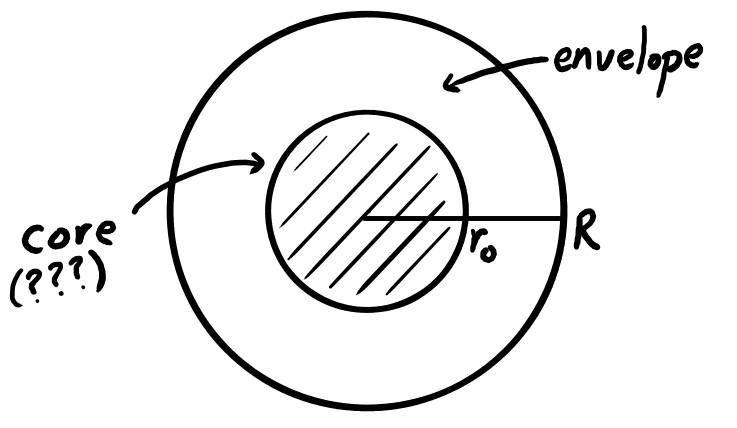
\includegraphics[width=0.75\textwidth]{2019/01/20190121_starcore.png}
    \caption{A schematic drawing of the interior $+$ envelope model for a star. The interior region extends from $0<r\leq r_0$ and the exterior region (envelope) goes from $r_0 < r < R$, to the surface of the star.}
    \label{fig:starcore}
\end{figure}

What could happen in the interior? If $\rho$ takes on some value $\rho(r_0)=\rho_0$ on the surface of the core, then by integrating we can put the bound
\begin{equation}
    m_0 \geq \frac{4\pi}{3} r_0^3 \rho_0
\end{equation}
on $m_0$ the mass contained in the core. That is, in the best case $\rho(r)$ is constant in the core region-- the star certainly cannot be less dense in its core. But we have another inequality on $m(r)$, the Buchdahl limit \ref{buchdahl}, which we can see is a decreasing function of $p$. So we evaluate this condition at $r=r_0,m(r_0)=m_0$, noting that the most general bound we can put on $m_0$ in terms of $r_0$ occurs when $p=0$. We find that
\begin{equation}
    \frac{m_0}{r_0} < \frac{4}{9}.
\end{equation}
These two inequalities in the space of core masses $m_0$ and core radii $r_0$ plus a value for the core density $\rho_0$ tell us that there is a limit on the total core mass-- taking $\rho_0= \SI{5e14}{\gram/\centi\meter^3}$, the density of nuclear matter, we find that $m_0<5 M_\odot$. Strictly, these are only limits on the core mass, but it turns out that the envelope region is generally insignificant, so
\begin{equation}
    M\approx m_0 < 5 M_\odot.
\end{equation}